\chapter{Przegląd piśmiennictwa}

Choroba Alzheimera nadal nie jest w pełni zrozumiana, jednak dzięki badaniom zdobyto już wiele istotnych informacji na jej temat.
Część z nich opiera się wyłącznie na korelacjach i potwierdzonych powiązaniach z pominięciem przyczyn i konkretnych mechanizmów nimi rządzących, lecz nadal daje nam to wystarczający obraz by przedstawić kompleksowo opis choroby.

\section{Historia, definicja i objawy choroby Alzheimera}

\subsection{Wczesna historia}

Istnienie demencji było znane ludzkości od bardzo dawna.
Pierwsze wzmianki na ten temat pojawiały się już w czasach starożytnej Grecji, a informacje dotyczące jej objawów można odnaleźć nawet wcześniej, w starożytnym Egipcie \cite{boller1998history}.

Natomiast choroba Alzheimera została po raz pierwszy opisana przez niemieckiego lekarza Aloisa Alzheimera, od którego nazwiska została później nazwana.
W roku 1901 neuropatolog zajął się przypadkiem Auguste Deter, pacjentki przyjętej do szpitala psychiatrycznego.
Od jej 51. roku życia zaczęły się stopniowe zmiany osobowości, które następnie przerodziły się w postępujące zaburzenia kognitywne, a ostatecznie w całkowitą apatię \cite{cipriani2011alzheimer}.
W momencie, gdy Alzheimer rozpoczął badania nad nią, pacjentka miała już prawie pięcioletnią historię narastających halucynacji, urojeń, apraksji, zaburzeń pamięci, mowy, społecznych i behawioralnych.

Po śmierci pacjentki lekarz przeprowadził badania mózgu zmarłej, w trakcie których znalazł zmiany i cechy dziś przypisywane omawianej chorobie.
Alzheimer przedstawił swoje kliniczne i patologiczne wyniki na konferencji południowo-zachodnich niemieckich psychiatrów w 1906 roku, następnie opublikował w formie pisemnej w czasopismach medycznych poświęconych psychiatrii \cite{alzheimer1906uber}.

W tym czasie jeszcze sam Alois Alzheimer nie był pewien, czy przypadek Auguste Deter reprezentował nowy zespół chorobowy.
Uważał, że opisał bardzo rzadką przypadłość i najprawdopodobniej wierzył, że była to po prostu szczególna forma demencji starczej \cite{cipriani2011alzheimer}.
Dopiero kilka lat później, po raz pierwszy użyty został termin ``choroba Alzheimera'' (\emph{ang. ``Alzheimer's disease'', często po prostu ``AD''}) w wydanym podręczniku psychiatrii Emila Kraeplina \cite{kraepelin1910psychiatrie}.

Jeszcze w pierwszej połowie XX wieku publikacje podkreślały brak zależności przebiegu choroby Alzheimera od wieku pacjentów.
Pojawiła się również istotna kliniczna debata wokół pytania czy demencja ``przedstarcza'' oraz demencja ``starcza'' (\emph{ang. kolejno ``presenile'' oraz ``senile''}) są tym samym zaburzeniem \cite{jellinger2006alzheimer}.
W połowie wieku pojawiły się pierwsze postulaty mówiące, że (przedstarcze) \emph{AD} oraz demencja starcza są całkowicie odrębnymi jednostkami chorobowymi (choć nowsze badania dojść jednoznacznie pokazują że tak nie jest).

W latach 60 XX wieku rozpoczęła się nowa era badań bazująca na nowym, bardzo ważnym narzędziu badawczym -- mikroskopii elektronowej.
Dzięki niej możliwe było zbadanie struktury komórek nerwowych i ich połączeń, a także zbadanie struktury i składu splotów nerwowych znajdujących się w mózgu.
Takich opisów jako jeden z pierwszych dostarczył w 1963 roku Kidd, który opisał zmiany w strukturze splątków neurofibrylarnych oraz blaszek amyloidowych \cite{kidd1963paired}.

Od tego czasu choroba progresywnie zyskiwała coraz większą uwagę ze strony środowiska naukowego, a także społeczeństwa.
W 1974 roku rząd Stanów Zjednoczonych Ameryki powołał do istnienia Narodowy Instytut ds. Starzenia się (\emph{ang. National Institute on Aging, NIA}), który od tego czasu finansuje badania nad chorobą Alzheimera \cite{marx1974aging}.
W 1980 roku powstało ``Stowarzyszenie Choroby Alzheimera i Pokrewnych Zaburzeń'' (\emph{ang. Alzheimer's Disease and Related Disorders Association, ADRDA}), organizacja non-profit, która dziś znana jest jako ``Stowarzyszenie Choroby Alzheimera'' (\emph{ang. Alzheimer's Association, AA}).
Wraz z rosnącą świadomością społeczną wzrastało także finansowanie, dzięki czemu choroba jeszcze 30 lat temu uznawana za całkiem nieuleczalną i nie do powstrzymania czy spowolnienia, dziś jest jedną z najbardziej intensywnie badanych chorób neurodegeneracyjnych z prospektami na walkę z nią w niedalekiej przyszłości.

Mimo tych wielu obecnych badań, nadal pozostaje wiele czynników wciąż niepoznanych i nie ma jednoznacznej odpowiedzi na pytanie co jest przyczyną choroby Alzheimera.
Wciąż brakuje również skutecznych metod leczenia, które mogłyby zatrzymać jej postęp lub spowolnić go w znaczący sposób.

\subsection{Współczesna definicja choroby Alzheimera}

W celu lepszego zrozumienia choroby Alzheimera, warto najpierw przyjrzeć się dwóm definicjom -- czym jest demencja oraz czym jest choroba Alzheimera -- jako, że terminy te często w świadomości publicznej są utożsamiane, co nie jest prawdą, choć pojawiają się miedzy nimi istotne powiązania.

Demencja (inaczej \emph{otępienie}) to znacznie ogólniejszy termin określający utratę pamięci, zdolności językowych, umiejętności rozwiązywania problemów i utrudnienie innych czynności poznawczych, które są na tyle poważne, że przeszkadzają w codziennym życiu.
Nie odnosi się w żadnym wypadku do naturalnego procesu starzenia się, i nie należy drobnych problemów z pamięcią czy zapominalstwa z nią mylić.
Demencja jest też objawem, a nie chorobą, i może być spowodowana przez wiele różnych chorób i zaburzeń.

Choroba Alzheimera jest jedną z wielu chorób, które mogą prowadzić do demencji.
Odpowiada ona za między 60\% a 80\% przypadków demencji, co czyni ją najczęstszą przyczyną otępienia \cite{what-is-alzheimers:2023}.
Obecnie klinicyści używają terminu \emph{AD} -- choroba Alzheimera -- w odniesieniu do zespołu chorobowego, który objawia się charakterystycznym postępującym zaburzeniem amnezyjnym z późniejszym pojawianiem się innych zmian poznawczych, behawioralnych i neuropsychiatrycznych, które upośledzają funkcje społeczne i czynności życia codziennego \cite{cummings2004alzheimer}.

Mimo, że choroba Alzheimera jest najczęstszą przyczyną demencji, to jednak nie jest z nią tożsama.
Drugą najczęstszą przyczyną jest demencja naczyniowa, która jest spowodowana uszkodzeniem naczyń krwionośnych w mózgu, najczęściej w wyniku udaru mózgu.


\subsection{Objawy choroby Alzheimera i stadium demencji}

Objawy choroby Alzheimera są bardzo zróżnicowane i zależą od stadium choroby.
Dodatkowo wczesne objawy często są mylone z naturalnym procesem starzenia się, co utrudnia wczesną diagnozę.

Ogólnie rzecz biorąc, objawy choroby Alzheimera można podzielić na 3 główne etapy powiązane ze stadium choroby \cite{alzheimers-symptoms:2021}:

\begin{itemize}

  \item Wczesne objawy

        W początkach rozwijającej się choroby głównym symptomem są zaniki pamięci.
        Można tutaj wymienić między innymi zapominanie o niedawnych rozmowach lub wydarzeniach, gubienie przedmiotów, zapominać nazw miejsc i rzeczy, powtarzanie się, trudności w znalezieniu właściwego słowa czy podejmowaniu decyzji.
        Łatwo zauważyć, że są to objawy, które mogą pojawić się w mniejszym stopniu u każdego człowieka, w tym w pełni zdrowego, co znacznie utrudnia wczesną diagnozę -- nasilenia się tych objawów są często mylone z naturalnym procesem starzenia się.

  \item Objawy w średnim stadium

        Narastają przypadku dezorientacji - na przykład gubienie się, błądzenie czy brak świadomości pory dnia.
        Chory może powtarzać czynności, mieć urojenia, odczuwać paranoję, zaburzony jest sen.
        AD może również wpływać na psychikę, powodując częste zachwiania nastroju, niepokój, frustrację czy depresję \cite{li2014behavioral}.
        Niebezpieczne mogą być także problemy z percepcją -- ocena odległości czy uświadamiane widzenie lub słyszenie.

        Wraz z rozwojem choroby Alzheimera, problemy z pamięcią będą się pogarszać.
        Pogłębiają się problemy z zapamiętywaniem imion, nawet tych osób, które zna się od dawna.
        Mogą pojawiać się także trudności w rozpoznawaniu miejsc i osób.
        Ciężkim, możliwym objawem pojawiającym się w średnim stadium jest także afazja, czyli zaburzenia mowy i języka.

        Na tym etapie osoba cierpiąca na chorobę Alzheimera zazwyczaj potrzebuje wsparcia w codziennym życiu.

  \item Późniejsze objawy

        W późniejszych stadiach choroby Alzheimera objawy stają się coraz bardziej nasilone i mogą być w znacznym stopniu wpływać na osobę chorą, a także jej opiekunów, przyjaciół i rodziny.

        Mogą pojawiać się halucynacje i urojenia, zanikające lub nasilające się wraz z postępem choroby.
        Czasami osoby cierpiące na chorobę Alzheimera mogą być agresywne, wymagające i podejrzliwe w stosunku do otoczenia.

        W miarę postępu choroby Alzheimera może również rozwinąć się szereg innych objawów, takich jak dysfagia (trudności z połykaniem), nietrzymanie moczu czy stolca, problemy z poruszaniem się bez pomocy, fizyczna utrata masy ciała, a także stopniowa i często szybka utrata zdolności poznawczych -- w tym mowy \cite{joe2019cognitive}.
        Znacznie pogłębiają się problemy z krótko- i długoterminową.

        W ciężkich stadiach choroby Alzheimera ludzie mogą potrzebować całodobowej opieki oraz pomocy w jedzeniu, poruszaniu się i pielęgnacji osobistej.

\end{itemize}

\section{Diagnoza choroby Alzheimera}

Mimo, że choroba Alzheimera nadal nie jest w pełni zrozumiana i zbadana oraz wciąż nie ma skutecznych metod jej leczenia, to obszar diagnozy i wczesnego wykrywania choroby jest bardzo dobrze rozwinięty.
Powstało wiele metod i narzędzi diagnostycznych, które pozwalają na wczesne wykrycie choroby.

\subsection{Metody kliniczne diagnostyki choroby Alzheimera}

Między rokiem 1960 a 1985 wprowadzono kilka różnych kategorii obiektywnych klinicznie narzędzi diagnostyki choroby Alzheimera, wiele z nich potwierdzonych w autopsji \cite{khachaturian2006diagnosis}.
Były to między innymi:

\begin{itemize}

  \item \emph{Mini-Mental State Examination} (w skrócie \emph{MMSE}, potocznie mini-mental) -- jest to zaprojektowany w 1975 roku test oceny demencji oraz jej stopnia w formie szybkiego badania, najczęściej krótszego niż 5 minut.
        Mini-mental jest narzędziem przesiewowym (ang. \emph{screening}), to jest -- nie jest dokładne i jednoznaczne, ale jego negatywny wynik daje podstawy przypuszczać prawdopodobną utratę zdolności kognitywnych i wszcząć
        głębsze, kliniczne badania w celu potwierdzenia wstępnej diagnozy.

        W wyniku tego badania uzyskuje się miedzy 0 a 30 punktów, gdzie wraz z malejącą zdobytą ilością rośnie domniemany stopień demencji.
        27 punktów oraz powyżej oznacza wynik prawidłowy, 24 i w górę to niedemenecyjne zaburzenia poznawcze, 19 wzwyż sugerują demencję łagodną, od 11 do 18 demencję średniego stopnia, a poniżej 10 demencję głęboką.

        Niedawne badania nad skutecznością MMSE na przestrzeni różnych kategorii stwierdzały jej czułość (sensitivity) między 23\% a 76\%, a jej specyficzność (specificity) między 40\% a 90\% \cite{arevalo2015mini}.
        Nie jest to więc wynik wysoki, jednakże wciąż jest to istotne narzędzie używane w praktyce klinicznej, głównie ze względu na jego prostotę i szybkość.

  \item \emph{Short Blessed Test} (w skrócie \emph{SBT}) -- badanie opublikowane do użytku w 1983 roku skupiające się na orientacji, pamięci i koncentracji \cite{katzman1983validation}.
        Według samych autorów przeznaczone do wykrywania wczesnych zaburzeń poznawczych, nie samej diagnozy choroby Alzheimera.
        Wszelkie wyniki sugerujące demencję wymagają dalszych badań.

  \item \emph{Clinician's Interview-Based Impression of Change plus caregiver input} (w skrócie \emph{CIBIC+}) -- zaproponowane i wymagane przez amerykańską Agencję Leków i Żywności (ang. \emph{FDA}, \emph{Food and Drug Administration}) podejście do przeprowadzania badań nad lekami na chorobę Alzheimera i demencję, który ma pozwalać na uzyskiwanie mierzalnych klinicznie danych potrzebnych do oceny skuteczności badanych środków \cite{joffres2000qualitative}.
        Najczęściej praktykowanym testem implementującym założenia CIBIC+ jest \emph{Alzheimer's Disease Cooperative Study -- Clinical Global Impression of Change} (w skrócie \emph{ADCS-CGIC}) z roku 1990.

  \item \emph{Clinical Dementia Rating} (w skrócie \emph{CDR}) -- skala numeryczna używana do ilościowego określenia nasilenia się objawów demencyjnych i skategoryzowania choroby w określonym "stadium".
        Wynik w tej skali otrzymuje się jako rezultat przeprowadzenia wywiadu z pacjentem opracowanego w 1993 roku przez Morrisa i jego współpracowników, lekarzy z Washington University School of Medicine \cite{morris1993clinical}.

        CDR uważany jest za test zdolny do rozpoznania bardzo łagodnych upośledzeń, co przeważnie nie było możliwe w poprzednich testach klinicznych dotyczących choroby Alzheimera.
        Ma on jednak słabe strony, w tym najważniejszy -- długi czas potrzebny na przeprowadzenie całościowego wywiadu, i co za tym idzie jest względnie niezdolny do uchwycenia zmian w czasie.
        Dodatkowo polega on na subiektywnej ocenie lekarza, co może prowadzić do błędów.

  \item \emph{Alzheimer's Disease Assessment Scale -- Cognitive Subscale} (w skrócie \emph{ADAS--Cog}) -- test kliniczny, który mierzy zmiany w funkcjonowaniu poznawczym pacjenta i nasilenie objawów demencji.
        Jest połową większego testu, \emph{Alzheimer's Disease Assessment Scale} (w skrócie \emph{ADAS}), który składa się z dwóch części: \emph{ADAS--Cog} oraz \emph{ADAS--Noncog}.
        ADAS--Cog zawiera 11 pytań, które oceniają pamięć, orientację, rozumienie, umiejętności wykonawcze i język.
        Do dnia dzisiejszego jest on na szeroką skalę używany w badaniach klinicznych nad lekami na demencję czy chorobę Alzheimera i uważany za najlepszy standard  ocenie leczenia przeciw otępieniu \cite{connor2008administration}.

\end{itemize}

Większość tego typu badań ma charakter niekonkluzywny i nie są w stanie jednoznacznie potwierdzić czy wykluczyć chorobę Alzheimera.
Wymagają one dalszych badań, które mogą być zarówno kliniczne, jak i laboratoryjne.
Część z nich jednak -- w szczególności ostatni z wymienionych, \emph{ADAS--Cog} -- są na tyle dokładne, że do dziś są bardzo szeroko używane w badaniach klinicznych nad chorobą Alzheimera.
A z kolei wszystkie są wystarczająco skuteczne, by być podstawą do podjęcia decyzji i przeprowadzeniu znacznie dokładniejszych badań laboratoryjnych.
Takimi dokładnymi badaniami biologicznymi mogą być pośmiertne badania neuropatologiczne, ale także możliwe jest w trakcie życia pacjenta badanie biomarkerów wskazujących na chorobę Alzheimera \cite{mantzavinos2017biomarkers}.

Nowoczesne uniwersalne narzędzia diagnostyczne są również bardzo przydatne w badaniach nad chorobą Alzheimera, w szczególności możliwość dokładnego obrazowania mózgu.

\subsection{Metody obrazowania mózgu w diagnostyce choroby Alzheimera}

Sugestie dotyczące przydatności i skuteczności nowych technik obrazowania mózgu w diagnostyce choroby Alzheimera pojawiły się już w latach 80 XX wieku \cite{mcgeer1986brain}.
Testowano wykorzystanie tomografii komputerowej (\emph{CT}), rezonansu magnetycznego (\emph{MRI}), pozytonowej tomografii emisyjnej (\emph{PET}) oraz pojedynczej emisji fotonów (\emph{SP}).
Autorzy wskazywali jednak, że skany tomografii komputerowej i rezonansu magnetycznego ujawniają uogólniony proces zanikowy kory mózgowej, który nasila się wraz z wiekiem i mimo, że proces zanikowy jest bardziej nasilony w chorobie Alzheimera, to jednak nie może być stosowany jako metoda diagnostyczna, ponieważ nie występuje w każdym przypadku.
Dodali też, że zmian nie można przewidzieć z użyciem tych dwóch wspomnianych metod.

Nowsze prace jednak nie są tak rygorystyczne w stosunku do metod obrazowania mózgu i zaznaczają, że zarówno pierwotnie używana tomografia komputerowa, a także następnie wprowadzony rezonans magnetyczny były i są z powodzeniem używane w diagnostyce choroby Alzheimera \cite{johnson2012brain}.
Co więcej, funkcjonalny rezonans magnetyczny (\emph{fMRI}) czy pozytonowa tomografia emisyjna (\emph{PET}) potrafiły wykazać charakterystyczne zmiany w mózgach pacjentów z \emph{AD} w stadiach nawet przedobjawowych,
Żadna z metod obrazowania nie może służyć wszystkim celom, ponieważ każda z nich ma unikalne mocne i słabe strony.

Bardzo świeże prace z 2022 roku opisują, że obecnie neuroobrazowanie znajduje się w ścisłej czołówce metod pomocnych w diagnozowaniu choroby Alzheimera (\emph{AD}), a także innych wszelkich innych rodzajów demencji, takich jak otępienie czołowo-skroniowe, otępienie naczyniowe i otępienie z ciałami Lewy'ego (\emph{DLB}) \cite{scheltens2022imaging}.
Niedawno sformułowane przez Dubois i współpracowników kryteria badawcze dla wczesnej choroby Alzheimera wyraźnie wymieniają obrazowanie rezonansu magnetycznego (\emph{MRI}) i pozytonową tomografię emisyjną (\emph{PET}) dla \emph{AD} i są przykładem rozwoju nowego procesu diagnostycznego.
Autorzy sugerują, że wkrótce neuroobrazowanie zostanie włączone do kryteriów diagnostycznych dla różnych rodzajów demencji.

\subsection{Nowoczesne metody detekcji choroby Alzheimera z użyciem uczenia maszynowego}

Diagnostyka choroby Alzheimera miała duże skoki rozwojowe wraz z powstawaniem nowych technologii i metod badawczych.
Już w połowie lat 90 XX wieku pojawiły się pierwsze prace naukowe próbujące wykorzystać rozwijającą się dziedzinę uczenia maszynowego przy detekcji demencji.
Te pierwsze próby opierały się jednak nie na obrazach, ale na analizie danych klinicznych i rezultatów testów psychometrycznych \cite{datta1996applying}.
Rezultaty pokazały, że już te proste podejścia mają skuteczność nieco lepszą niż kwestionariusze zaprojektowane do ręcznej analizy zebranych danych.

Rosnąca popularność neuroobrazowania w diagnostyce choroby Alzheimera oraz dalszy rozwój technik uczenia maszynowego i sztucznej inteligencji doprowadziły do powstania wielu prac naukowych, które łączą te dwa obszary.

W 2007 roku podjęto próbę analizy kształtu hipokampu u pacjentów z chorobą Alzheimera z użyciem technik uczenia maszynowego \cite{li2007hippocampal}.
W wyniku uznano, że subtelne i przestrzennie złożone wzorce deformacji hipokampa pomiędzy pacjentami posiadającymi AD a zdrowymi osobami kontrolnymi można wykryć za pomocą metod uczenia maszynowego.

Dalsze badania sprawdzały skuteczność technik klasyfikacji w uczeniu maszynowym obrazów rezonansu magnetycznego w celu detekcji choroby Alzheimera \cite{herrera2013classification}.
Klasyfikacja miała być binarna, czyli obrazy były przydzielane do kategorii osób zdrowych lub kategorii osób z chorobą Alzheimera, bez podziału na stadium choroby.
Powstały model miał służyć jako pomoc we wczesnym sygnalizowaniu potencjalnych wskaźników choroby Alzheimera.

Nowe prace analizowały wykorzystywane do celów diagnostyki metody uczenia maszynowego na przestrzeni lat 2005 do 2019 \cite{tanveer2020machine}.
Zamknięto pojawiające się techniki w 3 kategoriach: maszyny wektorów nośnych (ang. \emph{Support Vector Machine}, \emph{SVM}), sztuczne sieci neuronowe (ang. \emph{Artificial Neural Network}, \emph{ANN}) oraz uczenie głębokie (ang. \emph{Deep Learning}, \emph{DL}).
Jak się okazuje, najwięcej prac naukowych używało technik maszyn wektorów nośnych \emph{SVM} ze względu na ich powtarzalność i solidność wyników, nie cierpią one bowiem na problemy związane z lokalnymi minimami.
Jednak sieci neuronowe są bardziej wszechstronne jeśli chodzi o przyrostowe uczenie się i modelowanie danych sekwencyjnych.
Najbardziej obiecująca jednak była technika uczenia głębokiego, dzięki której można modelować bardzo złożone dane z dużą dokładnością.

W tę właśnie stronę poszli autorzy późniejszej pracy, którzy używając obrazów rezonansu magnetycznego MRI wyszkolili głęboki model dla detekcji choroby Alzheimera \cite{ebrahimi2021deep}.
Wykorzystali oni konwolucyjne głębokie sieci neuronowe i różne rodzaje sieci rekurencyjnych bazowanych na wstępnie wytrenowanym modelu ResNet-18.
Otrzymali bardzo obiecujące wyniki i model, który osiągnął maksymalną wydajność klasyfikacji z dokładnością, czułością i swoistością na poziomie około 92\%.

\section{Uczenie maszynowe i techniki klasyfikacji}

W celu lepszego zrozumienia dlaczego i w jaki sposób uczenie maszynowe może być bardzo przydatnym narzędziem w diagnostyce choroby Alzheimera, a także całym ogólniej w obszarze medycyny i diagnostyki, warto przyjrzeć się na czym polega i jakie są jego podstawowe techniki.

\subsection{Generalna definicja uczenia maszynowego}

Uczenie maszynowe (często w skrócie \emph{ML}, z ang. \emph{Machine Learning}) jest pojęciem bardzo szerokim i z natury interdyscyplinarnym, natomiast w najpopularniejszym użyciu odnosi się do kategorii sztucznej inteligencji, która pozwala komputerom ``myśleć'' i uczyć się we własnym zakresie.
Sam termin został po raz pierwszy użyty przez Arthura Samuela w 1959 roku, który to zdefiniował uczenie maszynowe jako dziedzinę studiów, która daje komputerom możliwość uczenia się bez ich bezpośredniego programowania \cite{samuel1959some}.

Taka definicja uczenia maszynowego, mimo, że ogranicza się do jednej z wielu dziedzin potencjalnie zaliczanych do tej kategorii, jest bardzo ogólna i nie precyzuje dokładnie co to znaczy ``uczyć się''. ani jak takie uczenie się miałoby być manifestowane.
Jest to zabieg celowy, ponieważ -- w przeciwieństwie do tego, co pozwalałyby sądzić najpopularniejsze obecnie metody uczenia maszynowego -- nie jest to jedynie zbiór badań nad sieciami neuronowymi i systemami ekspertowymi.
Wspomniana definicja jednak jest zbyt ogólna, by móc powiedzieć o niej coś więcej bez bazowania na przykładowych technikach i algorytmach.

Aby sformalizować pewne uniwersalne właściwości technik uczenia maszynowego, zaproponowany został podstawowy model uczenia maszynowego.
W nim uczenie maszynowe zostało zaprezentowane jako proces składający się z czterech głównych elementów: środowiska, uczenia, repozytorium oraz wykonania \cite{wang2009brief}.
Wygląd takiego modelu został przedstawiony na \hyperref[fig:basic-model-of-machine-learning]{rysunku \ref*{fig:basic-model-of-machine-learning}}.

\begin{figure}[ht]
  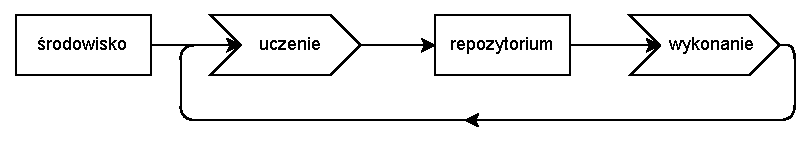
\includegraphics[width=\textwidth]{basic-model-of-machine-learning}
  \caption[Podstawowy model uczenia maszynowego]{Podstawowy model uczenia maszynowego zaadoptowany z pracy Hua Wang, Cuiqin Ma oraz Lijuan Zhou \cite{wang2009brief}. Bloki prostokątne oznaczają systemy a bloki procesowe (przypominające strzałki) oznaczają procesy.}
  \label{fig:basic-model-of-machine-learning}
\end{figure}

\begin{itemize}

  \item W modelu tym ``środowisko'' jest zewnętrznym zbiorem danych, które dostarczane są w pewnej bliżej nieokreślonej formie, reprezentuje źródła informacji zewnętrznych.
        Może to być na przykład zbiór obrazków przedstawiających odręcznie zapisane cyfry arabskie ręcznie oznaczonych rzeczywistą odpowiadającą im cyfrą przez człowieka.
        Mogą to być jednak także wszelkie inne dane pochodzenia zewnętrznego względem systemu uczenia maszynowego a które służą za podstawę do dalszego jego działania i kluczowego procesu uczenia się.


  \item Drugim czynnikiem tego modelu jest ``uczenie'', które jest procesem przetwarzającym informacje zewnętrzne na wiedzę.
        Terminy tutaj występujące są abstrakcją i mogą oznaczać wiele różnych rzeczy, w zależności od konkretnej omawianej techniki.
        Przykładowo w sztucznych sieciach neuronowych uczenie jest realizowane przez algorytm propagacji wstecznej błędu.
        Niezależnie od implementacji, wiedza jako szeroko pojęty rezultat uczenia jest trafia następnie do przechowania w repozytorium.

  \item Trzeci blok modelu, ``repozytorium'', jest miejscem przechowywania ogólnych zasad, które następnie kierują częścią działań wykonawczych systemu uczenia maszynowego.
        W przypadku sztucznych sieci neuronowych takim repozytorium jest sama struktura sieci oraz wagi połączeń między neuronami.
        Jest to szczególnie ciekawy przypadek, gdzie wiedza ta jest przechowywana w formie w zasadzie niedostępnej i niezrozumiałej dla człowieka, gdzie jej wydobycie jest bardzo trudnym zadaniem \cite{boger1997knowledge}.

  \item Ostatni blok modelu to ``wykonanie'', czyli proces, w którym system uczenia maszynowego wykorzystuje zgromadzoną w repozytorium wiedzę do podejmowania decyzji w kontekście problemu, który ma rozwiązać.
        Wynik działania procesu wykonawczego trafia później z powrotem do procesu uczenia, gdzie razem z dalszymi danymi pochodzącymi ze ``środowiska'' jest wykorzystywany do dalszego rozwoju wiedzy.

\end{itemize}

Cały proces zapętla się i pozwala na inkrementacyjne poprawianie wiedzy systemu uczenia maszynowego, aż do osiągnięcia pożądanej skuteczności procesu wykonawczego.
Tak przedstawiony model jest dużą abstrakcją pozostawiającą szczegóły implementacyjne i działania poszczególnych bloków poszczególnym technikom uczenia maszynowego, ale pozwala wyciąganie wniosków całościowych na temat uczenia maszynowego w pracach natury teoretycznej.

Jednak dążąc do lepszego poznania uczenia maszynowego od strony praktycznej, najlepiej jest przyjrzeć się kategoriom technik uczenia maszynowego, które są najczęściej wykorzystywane.

\subsection{Kategorie technik uczenia maszynowego}

Tradycyjnie wyróżnić można trzy paradygmaty ``uczenia'', na które dzieli się szerzej pojęte uczenie maszynowe.
Podział ten bazuje bezpośrednio na rozróżnieniu rodzajów sygnału -- danych dostarczanych do systemu uczenia maszynowego -- oraz informacji zwrotnej przekazywanej systemowi.
Te aspekty z kolei pośrednio wpływają na to, w jaki sposób w ogóle tego typu algorytm się zachowuje i jakie są jego możliwości oraz predyspozycje.
Kategorie te to:

\begin{itemize}

  \item \emph{Uczenie nadzorowane} (ang. \emph{supervised learning}) --
        algorytmy tego typu opierają się na analizie (czy przyswajaniu) zbiorów danych składających się zarówno z sygnału wejściowego, jak i opisanej już informacji zwrotnej.
        Dane wejściowe mogą być w dowolnej postaci, tekstowej, liczbowej, obrazkowej, dźwiękowej -- cokolwiek co może zostać zakodowane w sposób, w jaki algorytm reprezentuje dane.

        Co wyróżnia tę kategorię wśród pozostałych to fakt, że częścią danych przekazywanych do algorytmu jest także informacja na temat oczekiwanego wyjścia, zachowania się modelu.
        Przekazujemy algorytmowi to, jak powinien na podane dane wejściowe zareagować, a proces jego uczenia polega na dopasowaniu się do tych oczekiwań.

        Uczenie nadzorowane jest czasem nazywane także \emph{klasyfikacją} lub \emph{uczeniem indukcyjnym}, chociaż nie są to terminy ściśle równoważne.
        Pojawiają się jednak, ponieważ algorytmy tego typu przypominają rozumowanie indukcyjne, które polega na wyciąganiu ogólnych wniosków na podstawie konkretnych przykładów.
        Dodatkowo są szczególnie przydatne w zadaniach klasyfikacyjnych, w których radzą sobie bardzo dobrze \cite{hastie2009overview}.

        Do zadań klasyfikacyjnych wymagana jest możliwość podzielenia zbioru danych wejściowych na kategorie, gdzie każdy element przynależy do jednej z nich.
        Jednak uczenie nadzorowane także dobrze radzi sobie z problemami regresji, czyli przewidywania wartości liczbowych na podstawie danych wejściowych.
        Wtedy wyjściem nie jest dyskretna kategoria, ale liczba rzeczywista gdzie dozwolony jest pewien margines błędu -- algorytm ma dążyć jak najbliższej prawdziwej oczekiwanej wartości, jednak nie musi jej dokładnie osiągnąć.
        Przykładem może być system przewidywania cen nieruchomości na podstawie różnych cech mogących na nią wpływać.

        Systemu uczenia nadzorowanego nie potrafią jednak funkcjonować w izolacji -- potrzebują \emph{nadzoru}, zewnętrznej pomocy w postaci poprawnie opisanych lub skategoryzowanych danych wejściowych.
        W praktyce oznacza to, że uczenie nadzorowane jest zależne od człowieka, który musi dostarczyć algorytmowi dane wejściowe wraz z opisami, które często z angielskiego nazywane są \emph{labels}.
        Mimo skuteczności są więc ograniczane przez ilość danych, jaką jesteśmy w stanie dostarczyć, a także przez to, jak dobrze są one opisane.

        Popularnymi przykładami algorytmów uczenia nadzorowanego są między innymi \emph{regresja logistyczna} oraz \emph{k-najbliższych sąsiadów}.


  \item \emph{Uczenie nienadzorowane} (ang. \emph{unsupervised learning}) --
        systemy uczenia maszynowego tego typu różnią się od uczenia nadzorowanego w głównej mierze brakiem informacji zwrotnej.

        Otrzymują również zbiór danych wejściowych w dowolnej postaci, jednak nie są one opisane, nie wiemy odgórnie jak powinien zachować się algorytm na ich podstawie.

        Celem działania algorytmów uczenia nienadzorowanego jest znalezienie w nieopisanych danych wejściowych struktury i prawidłowości, na przykład ich zgrupowanie lub klasteryzacja (ang. \emph{clustering}) -- bezpośrednie wywnioskowanie bliżej nieokreślonych cech danych bez wsparcia z zewnątrz \cite{hastie2009unsupervised}.

        W uczeniu maszynowym tego typu w przeciwieństwie do uczenia nadzorowanego system zamiast reagować na informacje zwrotne powstałe poprzez porównanie opisu danych z wyjściem, algorytmy uczenia nienadzorowanego identyfikują podobieństwa w danych i reagują na podstawie obecności lub braku takich podobieństw w każdym nowym fragmencie zbioru wejściowego.

        Algorytmy uczenia nienadzorowanego są często wykorzystywane do analizy danych, w szczególności do wykrywania anomalii, czyli elementów zbioru danych, które wyróżniają się na tle pozostałych.

        Przykładem algorytmu uczenia nienadzorowanego jest algorytm centroidów, nazywany też algorytmem \emph{k-średnich} (ang. \emph{k-means}), który mimo swoich wad jest jednym z najpopularniejszych algorytmów klasteryzacji \cite{ahmed2020k}.
        Przez swoją nazwę jest często mylony lub błędnie utożsamiany z nadzorowanym podejściem k-najbliższych sąsiadów, jednak jest to zupełnie inny, niepowiązany algorytm.

  \item \emph{Uczenie przez wzmacnianie} (ang. \emph{reinforcement learning}) --
        podejście tego typu nieco różnią się od dwóch poprzednich, ponieważ nie są one zależne od predefiniowanego zbioru danych wejściowych, a od \emph{środowiska}, w którym algorytm się znajduje.
        Opierają się na ``nagradzaniu'' systemu za zachowania, które są pożądane i/lub ``karaniu'' za te niepożądane.

        Tym samym systemy takie są bliżej działania bazującego na modelu opartym na agentach (ang. \emph{agent-based model}, \emph{ABM}).
        Jest to model obliczeniowy służący do symulacji działań i interakcji autonomicznych agentów w celu zrozumienia zachowania systemu i tego, co rządzi jego wynikami.
        W omawianym kontekście oznacza to, że uczony przez wzmacnianie system jest traktowany jako ``agent'' w szeroko rozumianym środowisku, z którym wchodzi w różnego rodzaju interakcje.

        Ogólne założenia uczenia przez wzmacnianie przypominają nieco proces uczenia się, który widzimy u zwierząt i ludzi.
        Agent (system) jest umieszczany w środowisku, w którym może wykonywać pewne akcje.
        Wykonywane przez niego akcje prowadzą do pewnych rezultatów odbieranych przez niego jako nagrody lub kary.
        Otrzymywanie pozytywnych informacji zwrotnych -- nagród -- zachęca agenta do powtarzania akcji, które doprowadziły do ich otrzymania, a otrzymywanie negatywnych informacji zwrotnych -- kar -- zachęca do unikania prowadzących do nich czynności

        Agent skonstruowany jest tak, by chcieć maksymalizować otrzymywane nagrody, a minimalizować kary.
        Nazywane to jest funkcją nagrody (ang. \emph{reward function}).
        Dąży do tego sposobem, który w uproszczeniu można nazwać metodami prób i błędów.

        Przykładem algorytmów uczenia przez wzmacnianie jest metoda Monte Carlo.
        Jest to metoda statystyczna, która wykorzystuje powtarzalne losowania do rozwiązywania problemów, których rozwiązanie jest trudne lub niemożliwe do znalezienia w inny sposób.
        Agent ``próbkuje'' wykonywanie pewnej akcji i uśrednia uzyskane rezultaty -- wartości nagród/kar.
        Następnie uśredniony rezultat osiągnięty w trakcie trwania całości ``epizodu'', czyli pewnego konkretnego zdarzenia, jest wykorzystywany do zmiany zachowania agenta w przyszłości \cite{thrun2000reinforcement}.

\end{itemize}

W kontekście detekcji różnych jednostek chorobowych w medycynie, w tym choroby Alzheimera, najczęściej wykorzystywane są techniki uczenia nadzorowanego.
Pomimo, że uczenie nienadzorowane również dobrze sprawdza się w niektórych przypadkach \cite{raza2021tour} oraz uczenie przez wzmacniane także znajduje swoje zastosowania \cite{zhou2021deep}, to uczenie nadzorowane nadal sprawuje się najlepiej ze względu na naturę danych i problemów jakie najczęściej się w tym obszarze pojawiają.

Warto także dodać, że najnowsze popularne i bardzo obiecujące podejście -- tak zwane \emph{samo-nadzorowane uczenie maszynowe} (ang. \emph{self-supervised machine learning}) -- jest w istocie połączeniem technik uczenia nadzorowanego i nienadzorowanego i jest w stanie wykorzystać zalety obu tych podejść \cite{krishnan2022self}.

\subsection{Podstawowe algorytmy klasyfikacji}

\begin{itemize}
  \item Regresja logistyczna: klasyfikacja binarna
  \item \emph{K}-najbliższych sąsiadów (\emph{k-nn}): klasyfikacja oparta na podobieństwie
\end{itemize}

\subsection{Uczenie głębokie i sieci neuronowe}

\begin{itemize}
  \item Podstawy sieci neuronowych i neuronów
  \item Wpływ warstw neuronowych na zdolność modelu do abstrakcji
\end{itemize}

\subsection{Wykorzystanie konwolucyjnych sieci neuronowych}

\begin{itemize}
  \item Struktura i działanie sieci konwolucyjnych
  \item Przykłady zastosowań w analizie obrazów i diagnostyce medycznej
\end{itemize}

\subsection{Uczenie transferowe i wstępnie wytrenowane modele sieci neuronowych}

\begin{itemize}
  \item Zalety wykorzystania wstępnie wytrenowanych modeli
  \item Architektura przykładowego modelu
  \item Przeszkolenie i dostosowanie modelu do konkretnej analizy
\end{itemize}
